\section{Motivo della scelta}

La scelta dell’offerta è stata determinata da una combinazione di motivazioni personali e professionali, valutate in modo sistematico per garantire che l’esperienza di stage fosse 
coerente con i miei obiettivi di apprendimento e con le esigenze del corso di studi. Di seguito riporto i criteri che ho considerato e come li ho applicati nella selezione.

In primo luogo ho privilegiato la dimensione e la composizione del team: preferisco inserirsi in gruppi relativamente piccoli (4–10 persone) perché favoriscono una maggiore 
esposizione a responsabilità tecniche reali, feedback frequenti e contatto diretto con i tutor o i referenti tecnici. Nei team più piccoli è più probabile poter seguire 
un’intera feature dalla progettazione al rilascio, cosa che ritenevo fondamentale per un tirocinio formativo.

Ho dato poi grande importanza alla flessibilità della modalità di lavoro. Le posizioni che offrivano opzioni ibride o completamente remote hanno ricevuto una priorità maggiore, 
sia per motivi logistici sia perché consentivano di conciliare un possibile domani lavorativo nell'azienda ospitante con mia filosofia di vita. 
In fase di valutazione ho verificato sui profili LinkedIn e nelle descrizioni delle 
offerte la policy aziendale sul lavoro da remoto, la frequenza minima richiesta in presenza (es. 1–2 giorni a settimana) e la disponibilità a concordare orari flessibili.

Un altro fattore rilevante è stato l’allineamento tecnico e contenutistico del progetto con i miei interessi: ho preferito proposte che permettessero di lavorare su tecnologie 
affini alle mie preferenze circa l'intelligenza artificiale. 
Progetti che prevedevano l’uso di \emph{LLM}, \emph{RAG} o strumenti di orchestrazione agentica sono stati valutati positivamente perché avrebbero consentito di mettere in pratica competenze 
teoriche e sperimentare soluzioni rilevanti per il settore.

La logistica ha influenzato la decisione: ho considerato la distanza dalla sede più vicina e i tempi di spostamento stimati 
(in modo da non superare una soglia pratica per la presenza in ufficio) e la facilità di accesso con i mezzi pubblici. 
Nei casi in cui l’azienda avesse più sedi, ho valutato la sede operativa prevista e la relativa reperibilità.

Ambiti pratici come la possibilità di trasformare lo stage in una collaborazione successiva, la presenza di posizioni aperte per neo-laureati e 
la reputazione dell’azienda in termini di formazione interna sono stati considerati come elementi di prospettiva a medio termine. Anche la trasparenza su aspetti contrattuali 
(indennità di stage, durata, orari) ha inciso sulla scelta, benché non fosse l’unico criterio determinante.

\begin{figure}[htbp]
    \centering
    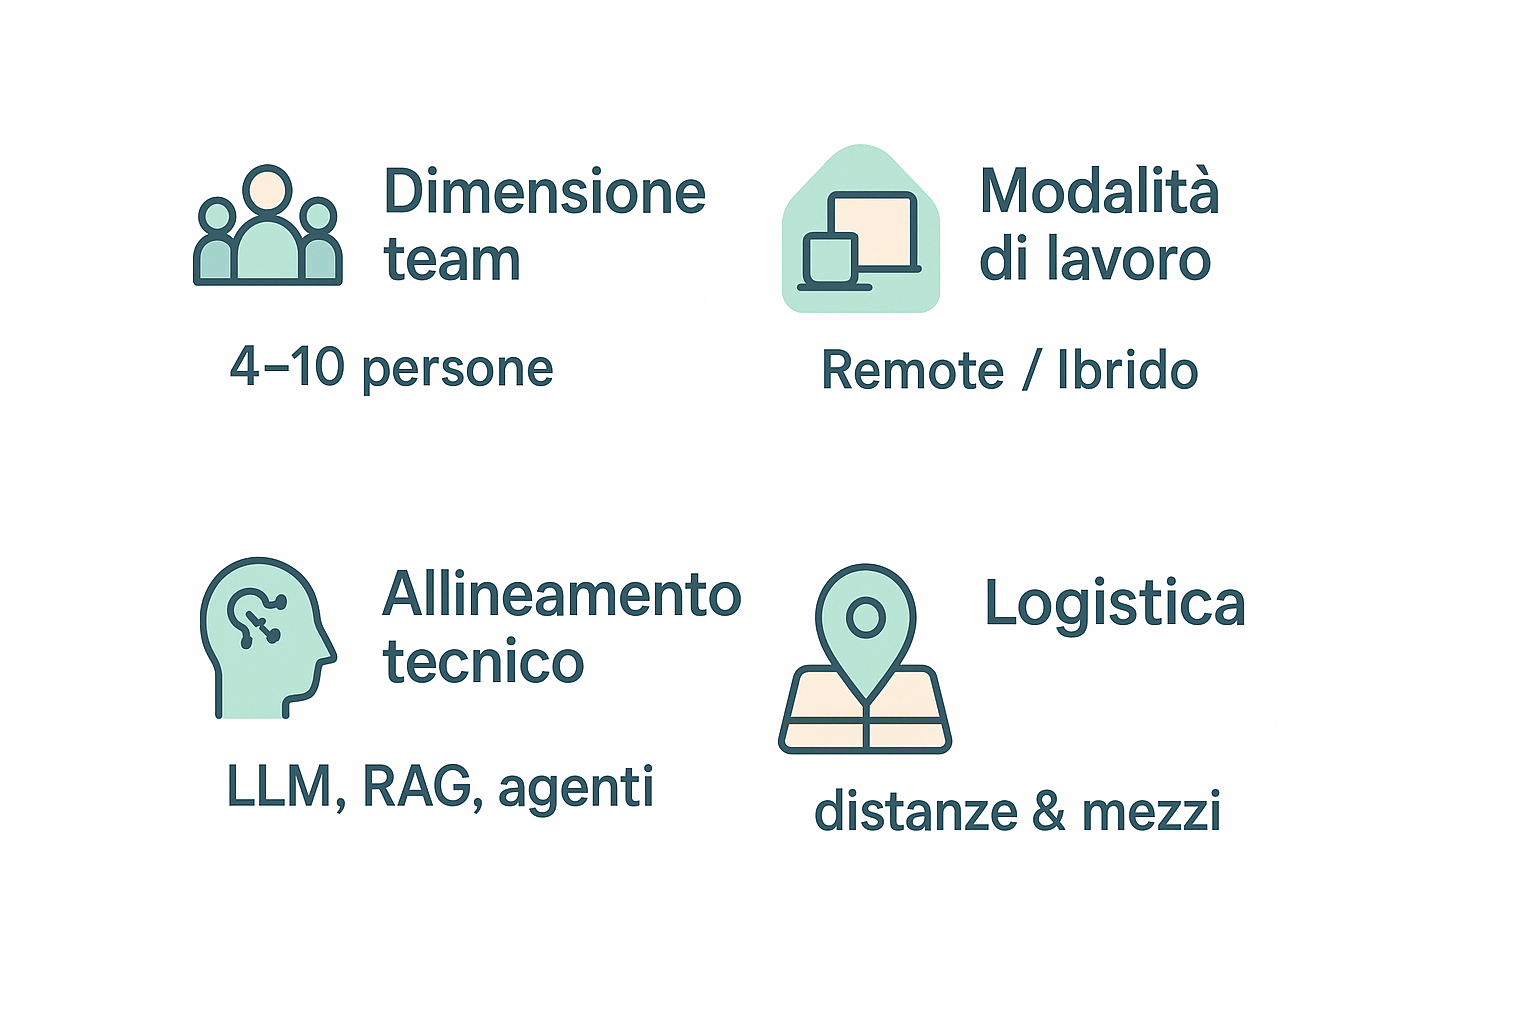
\includegraphics[width=0.8\textwidth]{stage/motivo}
    \caption{Criteri che hanno guidato la scelta dell’offerta.}
    \label{fig:motivo}
\end{figure}
%da ampliare

%Sotto-sezione in cui verrà descritto il motivo per cui ho preferito scegliere di fare lo stage presso questa azienda rispetto ad altre, 
%quali sono i miei obiettivi personali che mi sono auto-assegnato nello svolgimento del progetto e come si interconnettono con gli obiettivi dell'azienda.
%la ragione per la quale lo hai preferito alle altre offerte